\chapter{E2E Test Framework}
\label{chap:e2e-test-framework}

\section{Automated E2E Testing}
\label{sec:automated-e2e-testing}

\subsection{Manual vs Automatic E2E Testing}
\label{sec:manual-vs-automatic-e2e-testing}

\subsection{Technologies Used}
\label{sec:technologies-used}

\section{Test Framework Components}
\label{sec:test-framework-components}

\subsection{Feature Definition as Requirements}
\label{subsec:feautre-definition-as-requirements}

Feature files can be seen as an entry point to cucumber test cases \cite{featurefile1}. Each of the feature file should be written to test a single feature of the application or a particular area of feature \cite{featurefile2}. Since we were writing E2E tests for the payment feature, we created \texttt{buycredits.feature} file for testing this aspect. Consider \textbf{Listing \ref{lst:buycredits-feature-file}}:\\

\begin{listing}[H]
\begin{minted}[xleftmargin=\parindent, linenos, breaklines, breakanywhere, bgcolor=lightgray, fontsize=\small]{cucumber}
@dev @experiment
Feature: Buying Credit feature
  As a user of Synote
  I should be able to successfully buy credits when logged in

  Scenario: Access buy credits page when logged in
    Given I click the "Profile" button on "SideMenu" page
    Given I click the "BuyCredit" button on "Profile" page
    Then I should be on "BuyCredits" page

  Scenario: Buy credit with empty card number
    Given I click the "Profile" button on "SideMenu" page
    Given I click the "BuyCredit" button on "Profile" page
    Given I Correctly type in my details but "" for "number"
    Then Submit button should be disabled
//code omitted
\end{minted}
\captionof{listing}{Section of \texttt{buycredits.feature} file}
\label{lst:buycredits-feature-file}
\end{listing}

The section in \textbf{Listing \ref{lst:buycredits-feature-file}} is written in a language called \texttt{Gherkin}. \texttt{Gherkin} makes use of Business Readable Domain Specific Language (BRDSL) which allows us to write the test cases at a business level without getting into implementation details. 

Our client required us to document the requirements/specification for the new payment feature. Most of Synote's team are developers and since the feature file used \texttt{Gherkin}, it was readable on a business level and could act as automation test script \cite{featurefile1}. Hence, we recommended using the feature files themselves as the requirements documentation.\\

Each of the feature file should be defined with \texttt{Feature} keyword which consists of a name  (see \textbf{Listing \ref{lst:buycredits-feature-file}} line  2) and brief description  (see \textbf{Listing \ref{lst:buycredits-feature-file}} line  3-4). Each of the test cases are defined with \texttt{Scenario} keyword followed by a brief description of that test (see \textbf{Listing \ref{lst:buycredits-feature-file}} line  6 and 11). Each scenario should \cite{featurefile3}:
\begin{itemize}
\item Describe event taking place
\item Describe expected result
\end{itemize}

We use \texttt{Steps} to achieved this. Consider the \texttt{Access buy credits page when logged in} scenario in \textbf{Listing \ref{lst:buycredits-feature-file}}. We use keywords such as \texttt{Given} (line 7 and 8), \texttt{Then} (line 9) for writing readable test cases. Consider \textbf{Table \ref{tab:steps-keywords}} which define \texttt{Step} keywords \cite{featurefile1}

\begin{center}
%Column widths dependent on page width/margins
\begin{tabular}{ |p{2cm}|p{7cm}| }

 \hline
 	Keyword &
 	Description\\
 \hline
 	Given & Describes test pre-condition\\
 \hline
 	And & Defines additional test conditions\\
 \hline
 	Then & Defines expectations of test \\
 \hline

\end{tabular}
\captionof{table}{\texttt{Step keywords}}
\label{tab:steps-keywords}
\end{center}

\subsection{Reusable Steps Definition}
\label{subsec:reusable-steps-definition}

Cucumber is not able to execute the scenarios as they are. Instead, we have to write \texttt{step} definitions. Step definitions use regular expression to map the \texttt{Gherkin steps} to actions which will drive system interactions \cite{stepfile1}. Each of the \texttt{steps} written for scenarios in the \texttt{feature} file should have a \texttt{step} definition declared in its corresponding \texttt{step} file.\\ A \texttt{step} file should only contain definitions for \texttt{steps} used in corresponding \texttt{feature} file.\\

Consider \textbf{Listing \ref{lst:buycredits-step-file}}:\\

\begin{listing}[H]
\begin{minted}[xleftmargin=\parindent, linenos, breaklines, breakanywhere, bgcolor=lightgray, fontsize=\small]{cucumber}
@dev @experiment
//code omitted
	this.Given(/^I click the "([^"]*)" button on "([^"]*)" page$/, function (buttonName, pageName) {
        return this.Support.clickButton(buttonName, pageName);
    });

    this.Given(/^I should be on "([^"]*)" page$/, function (pageName) {
        return this.Support.waitUntil(this.Support.urlChanged(this.Support.getPageUrl(pageName)), 2000)();
    });
//code omitted
\end{minted}
\captionof{listing}{Section of \texttt{buycredits.steps.js} file}
\label{lst:buycredits-step-file}
\end{listing}

In our case, all the \texttt{steps} written in \texttt{buycredits.feature} file are defined in the \texttt{buycredits.steps.js} file. Each step should have a unique definition else an \texttt{ambiguous match} exception will be thrown. \textbf{Listing \ref{lst:buycredits-step-file}} contains the step definitions for \texttt{Access buy credits page when logged in} scenario in \textbf{Listing \ref{lst:buycredits-feature-file}}. Inside the step definitions, we write javascript code to handle the interaction logic e.g. 1st definition in \textbf{Listing \ref{lst:buycredits-step-file}} (line 3) handles clicking of button provided  \texttt{buttonName and pageName} parameters and 2nd definition (line 7) handles checking we are on a page with certain URL provided  \texttt{pageName} parameter. Nearly all of out step definitions take parameters instead of hard-coding them. This way, we can satisfy the \texttt{DRY} principle by reusing generic step definitions, making both  \texttt{feature} and  \texttt{step} files easily maintainable and readable in the long run.\\ 

\subsection{Reusable Support Functions}
\label{subsec:reusable-support-functions}

In order to have generic \texttt{step} definitions (e.g. see \textbf{Listing \ref{lst:buycredits-step-file}} line 3 and 7), we needed to write common generic methods which will drive interactions with the system. We place such functions in the \texttt{support.js} file. As a rule of thumb, we identified generic methods to go in the \texttt{support.js} file by checking if were were repeating any code/logic in the \texttt{bycredits.steps.js} file. Currently, our frame work uses the \texttt{support.js} file for:\\

\begin{itemize}
\item Clicking
\item Filling inputs
\item Navigating
\item Data retrieval
\end{itemize}

\begin{listing}[H]
\begin{minted}[xleftmargin=\parindent, linenos, breaklines, breakanywhere, bgcolor=lightgray, fontsize=\small]{cucumber}
@dev @experiment
//code omitted
	function loadPageOnSupport(pageName) {
    	if (!support[pageName]) {
        	support[pageName] = require('../pages/' + pageName.toLowerCase() + '.page.js');
    	}
	}
//code omitted
	fillInputOnPage: function (pageName, textBox, text) {
        loadPageOnSupport(pageName);
        if (this[pageName] && this[pageName][textBox + 'Input']) {
            var _textBox = this[pageName][textBox + 'Input'];
            return _textBox.sendKeys(text);
        }
    },
//code omitted
\end{minted}
\captionof{listing}{Section of \texttt{support.js} file}
\label{lst:support-file-methods}
\end{listing}

Consider \textbf{Listing \ref{lst:support-file-methods}}. The \texttt{fillInputOnPage} is a common generic method i.e. it can be used to fill any input field on any page, hence its placement in the \texttt{support.js} file. The \texttt{loadPageOnSupport} method helps \texttt{support.js} file to be generic in applying its methods in different contexts by dynamically requiring desired pages objects. Main advantage of \texttt{support.js} is that testers will never have to rewrite any code they have already written, satisfying the \texttt{DRY} principle.\\
\subsection{Pre and Post Hooks}
\label{subsec:pre-and-post-hooks}

\subsection{Page Objects}
\label{subsec:page-objects}
There are few key interactions which are very common throughout the application e.g. clicking buttons, filling in inputs, navigating to pages etc. It seemed tedious and time consuming to actually write separate methods for these interactions on different pages. We came to the conclusion that the interactions themselves should be generic enough so they can be applied to any page. The pages of application differed in the elements and components they had. Hence, we have definitions of \texttt{Page Object Models} which is composed of elements a page has. 

\begin{minipage}{.5\textwidth}
\begin{listing}[H]
\begin{minted}[xleftmargin=\parindent, linenos, breaklines, breakanywhere, bgcolor=lightgray, fontsize=\small]{js}
Title : "BuyCredits",
//code omitted
    Url : browser.deployment.hostUrl + 'buycredit',
    billing_nameInput : element(by.model('billingName')),
    numberInput : element(by.model('cardNumber')),
    cvcInput : element(by.model('cardCVC')),
    exp_monthInput : element(by.model('expMonth')),
    exp_yearInput : element(by.model('expYear')),
    PaySavedRadioButton : element(by.id('pay-saved-radio')),
//code omitted
  \end{minted}
  \captionof{listing}{Section of \texttt{buycredits.page.js} file}
  \label{lst:buycredits-page-code}
  \end{listing}
\end{minipage}%

\begin{figure}[!hbt]
  	\centering
 	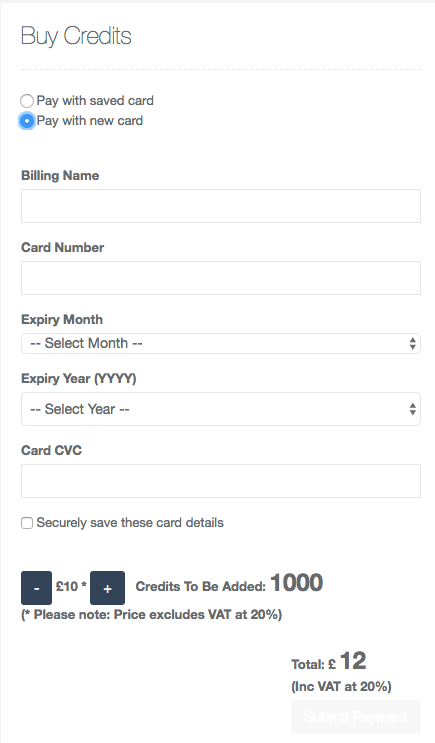
\includegraphics[width=0.6\textwidth]{screenshot-payment-form.png}
  	\caption{Payment Form}
 	\label{fig:paymentform-screenshot}
\end{figure}

Here you have the \texttt{buycredits.html} page (\textbf{Figure \ref{fig:paymentform-screenshot}}) and it has a corresponding \texttt{buycreditspage.js} \texttt{page object file} (\textbf{Listing \ref{lst:buycredits-page-code}}) which is basically a one to one mapping from the html page components. Page object files also house methods to interact with elements (defined in the same \texttt{page object model}) which are only applicable to the particular page in question e.g. \texttt{buycreditspage.js} has a method called \texttt{fillDefaultCardDetails} which fills in the payment form fields and is only applicable to \texttt{buycredits.html} page. The main advantages of implementing \texttt{page object models} was reduced code duplication and easy maintainability i.e.  if any of the UI element of the application was changed, we only have to modify them in the \texttt{page object} file instead of fixing them  in each \texttt{step} which used that UI element \cite{semaphore}. Another advantage is that it structures the framework, improving readability.\\ 
\subsection{Deployment Definition}
\label{subsec:deployment-definition}
One of the requirements of our client was that our framework should be capable of running the E2E test suite against different deployments of Synote. Then main concern we had here was that tests which worked on one deployment may not work on another deployment. To overcome this issue, we created 

Framework is capable of defining the actual deployment of Synote application to test against. I was one of the requirements we had to run the tests on different deployments. Things which worked on one deployment may not work on another deployment. 

This file defines the deployment 
So how do u actually define a deployment. Deployment is actually defined by different parameters, for example your host urls will be different for development machines to the actual deployment of the application. For example on the screen you seen a dev deployment which has different host url to experiment deployment. Also with cards, you would want to use a test card on test deployment and a live card on the live deployment. 

So it time consuming to manually enter all these data when you wanna test against a deployment. So u don’t do that. You define what a deployment is in the file called environment.js. and you pass in a parameter to that deployment reference to say which deployment I wanna run the tests against. This will setup the setting for you.  




\subsection{Reporting}
\label{subsec:reporting}

\subsection{Assessment}
\label{subsec:assessment}
